% Illustration for the slide "Hypothesis testing": common forms of H0 / Ha on the parameter line,
% Compile from class3/:  pdflatex hypotheses_forms.tex
%   then: pdftocairo -png -transp -singlefile -scale-to-x 2400 -scale-to-y -1 hypotheses_forms.pdf img/hypotheses_forms
\documentclass[tikz,border=4pt]{standalone}
\usepackage[T1]{fontenc}
\usepackage{lmodern}
\usepackage{amsmath,amssymb}
\usetikzlibrary{arrows.meta}
\definecolor{cnull}{HTML}{6A5ACD}
\definecolor{calt}{HTML}{EB078E}
\definecolor{cpharma}{HTML}{06BCF1}
\definecolor{cearth}{HTML}{8BB174}
\definecolor{txt}{RGB}{85,85,85}
\begin{document}
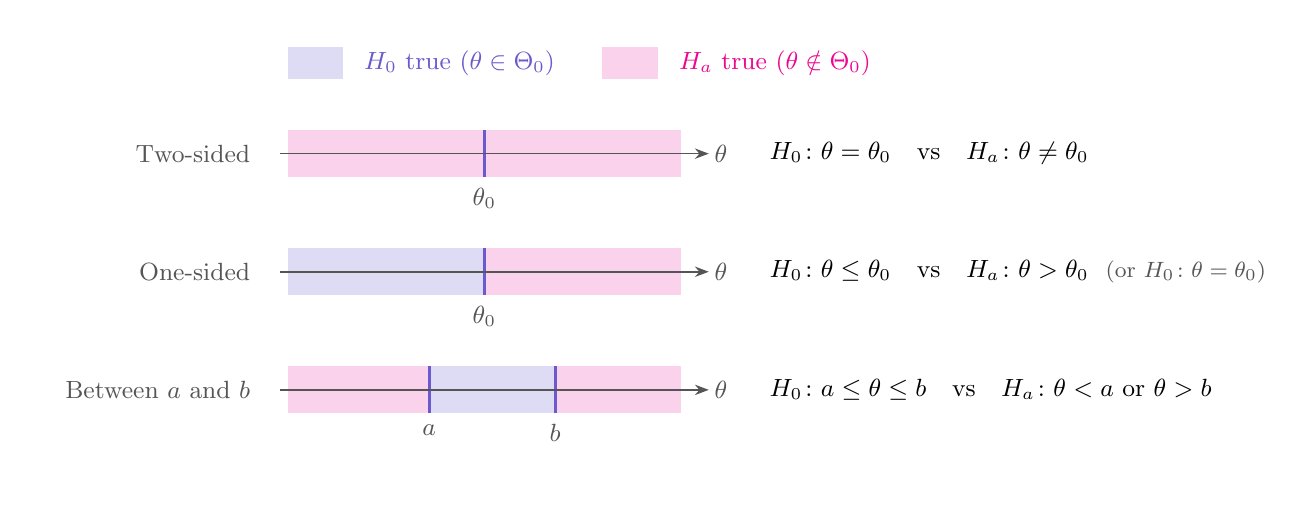
\begin{tikzpicture}[x=1cm,y=1cm,
  axis/.style={txt, line width=0.6pt, -{Stealth[length=5pt]}},
  b0/.style={fill=cnull!22, draw=none},
  ba/.style={fill=calt!18, draw=none},
  boff/.style={fill=gray!10, draw=none},
  cut/.style={cnull, line width=1.2pt},
  tick/.style={txt, font=\small, below=9pt},
  lab/.style={txt, anchor=east, font=\small},
  hyp/.style={anchor=west, font=\small},
  ex/.style={txt, anchor=west, font=\footnotesize}]
\useasboundingbox (-3.3,-0.55) rectangle (12.7,5.2);
\def\hb{0.3}   % half height of the bands

% legend
\fill[b0]  (0,4.55) rectangle (0.7,4.95);   \node[hyp, text=cnull] at (0.85,4.75) {$H_0$ true ($\theta \in \Theta_0$)};
\fill[ba]  (4.0,4.55) rectangle (4.7,4.95); \node[hyp, text=calt]  at (4.85,4.75) {$H_a$ true ($\theta \notin \Theta_0$)};

% 1. two-sided -------------------------------------------------------------
\def\y{3.6}
\node[lab] at (-0.35,\y) {Two-sided};
\fill[ba] (0,\y-\hb) rectangle (5,\y+\hb);
\draw[cut] (2.5,\y-\hb) -- (2.5,\y+\hb);
\draw[axis] (-0.1,\y) -- (5.35,\y); \node[txt, font=\small, anchor=west] at (5.3,\y) {$\theta$};
\node[tick] at (2.5,\y) {$\theta_0$};
\node[hyp] at (6.0,\y) {$H_0\colon \theta = \theta_0 \quad\text{vs}\quad H_a\colon \theta \neq \theta_0$};

% 2. one-sided -------------------------------------------------------------
\def\y{2.1}
\node[lab] at (-0.35,\y) {One-sided};
\fill[b0] (0,\y-\hb) rectangle (2.5,\y+\hb);
\fill[ba] (2.5,\y-\hb) rectangle (5,\y+\hb);
\draw[cut] (2.5,\y-\hb) -- (2.5,\y+\hb);
\draw[axis] (-0.1,\y) -- (5.35,\y); \node[txt, font=\small, anchor=west] at (5.3,\y) {$\theta$};
\node[tick] at (2.5,\y) {$\theta_0$};
\node[hyp] at (6.0,\y) {$H_0\colon \theta \leq \theta_0 \quad\text{vs}\quad H_a\colon \theta > \theta_0$ \ {\footnotesize\color{txt}(or $H_0\colon \theta = \theta_0$)}};

% 3. between a and b -------------------------------------------------------
\def\y{0.6}
\node[lab] at (-0.35,\y) {Between $a$ and $b$};
\fill[ba] (0,\y-\hb) rectangle (1.8,\y+\hb);
\fill[b0] (1.8,\y-\hb) rectangle (3.4,\y+\hb);
\fill[ba] (3.4,\y-\hb) rectangle (5,\y+\hb);
\draw[cut] (1.8,\y-\hb) -- (1.8,\y+\hb); \draw[cut] (3.4,\y-\hb) -- (3.4,\y+\hb);
\draw[axis] (-0.1,\y) -- (5.35,\y); \node[txt, font=\small, anchor=west] at (5.3,\y) {$\theta$};
\node[tick] at (1.8,\y) {$a$}; \node[tick] at (3.4,\y) {$b$};
\node[hyp] at (6.0,\y) {$H_0\colon a \leq \theta \leq b \quad\text{vs}\quad H_a\colon \theta < a \ \text{or}\ \theta > b$};
\end{tikzpicture}
\end{document}
